\begin{minipage}[t]{120mm}
\vspace{3mm}

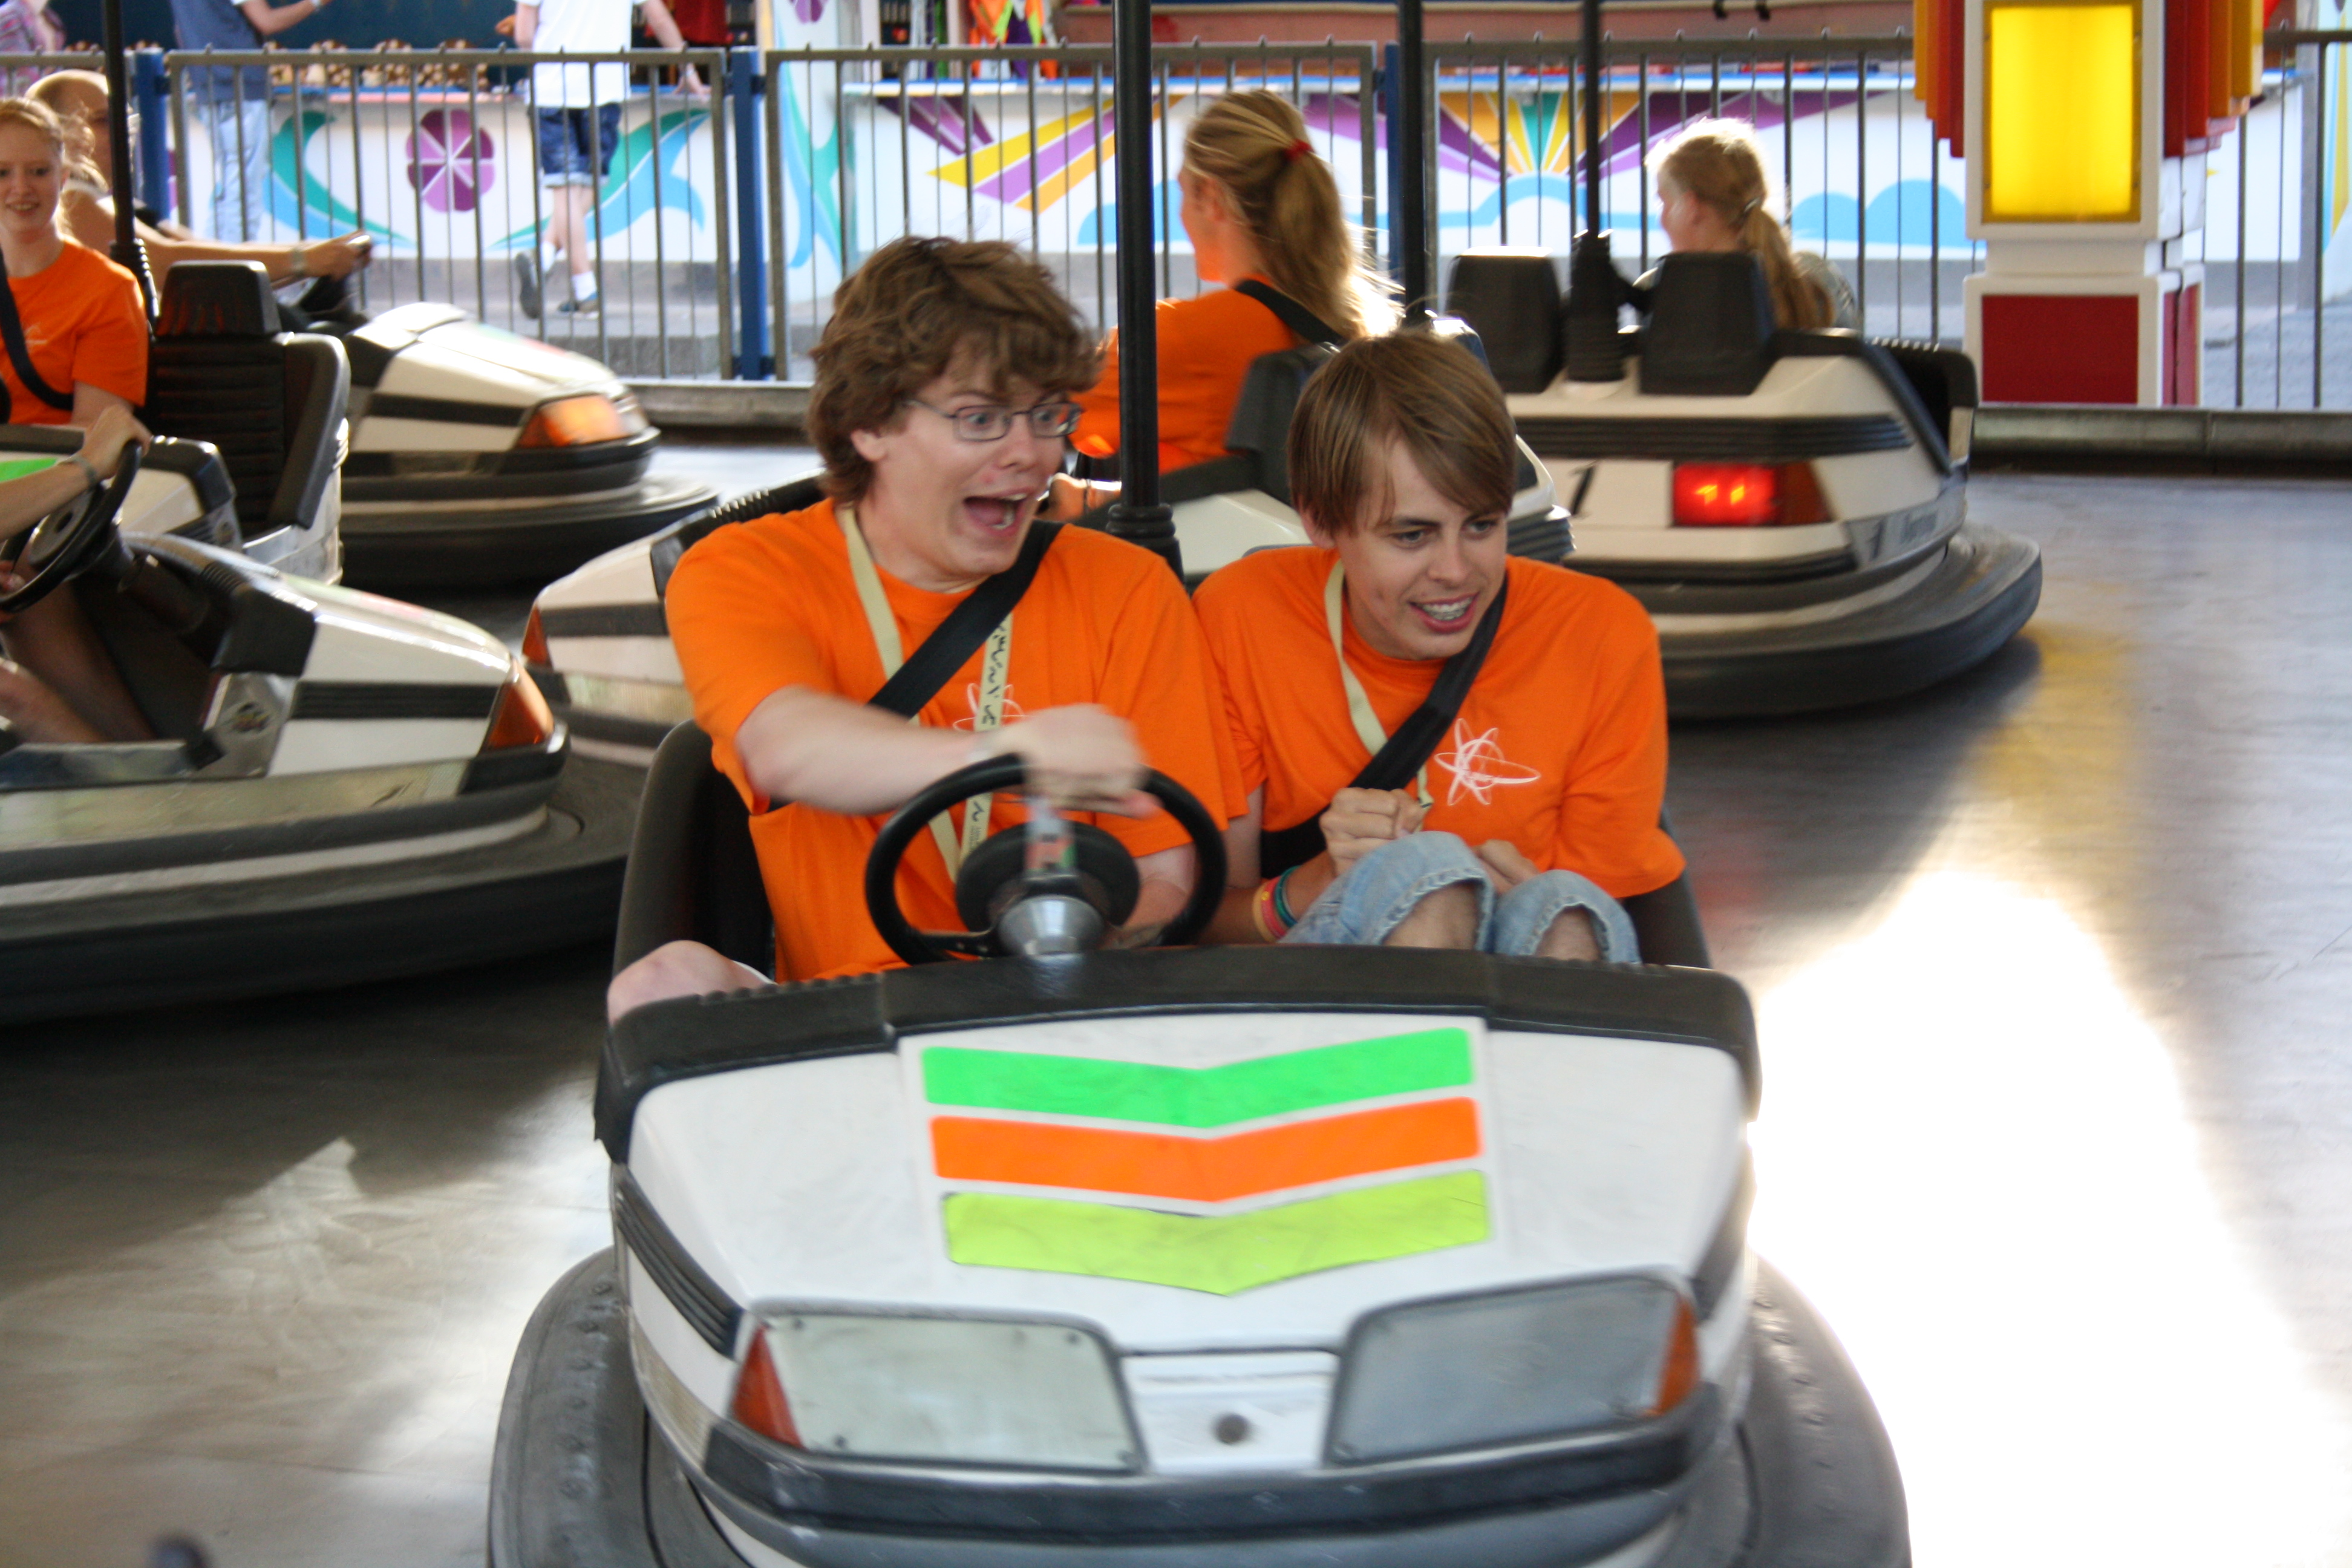
\includegraphics[width=\linewidth]{radiobil3.jpg}

\section*{Ikke-kommutativ studenterrådgivning}
\emph{Kære brevkasse}

Hvorfor er jeg så ked af det, og samtidigt så glad i dag?

\emph{Hilsen, en forvirret person}

\subsection*{Svar}

Du har tydeligvis været på camp, så dine følelser er helt almindelige. Glæden over en spændende og hyggelig uge, møder glæden til en hel nats søvn i en rigtig seng, og gør dig euforisk. Samtidigt ved du, at du så snart du tager afsked med dine medcampere på en station ude i landet, vil starte med at savne dem. Men frygt ikke, det er muligt at have kontakt med dem, også uden for en camp, og desuden vil der sikkert komme en ny camp i et nyt år, som man kunne deltage i igen, enten som deltager, hvis stadig man er så ung, som man plejede at være, og ellers måske som arrangør, hvis man begynder at være olding.

Så frygt ikke, livet går videre, på trods af. at det sikkert ikke er med samme grad af obskuritet.

{\flushright\emph{Hilsen den ikke-kommutative studenterrådgivning}}

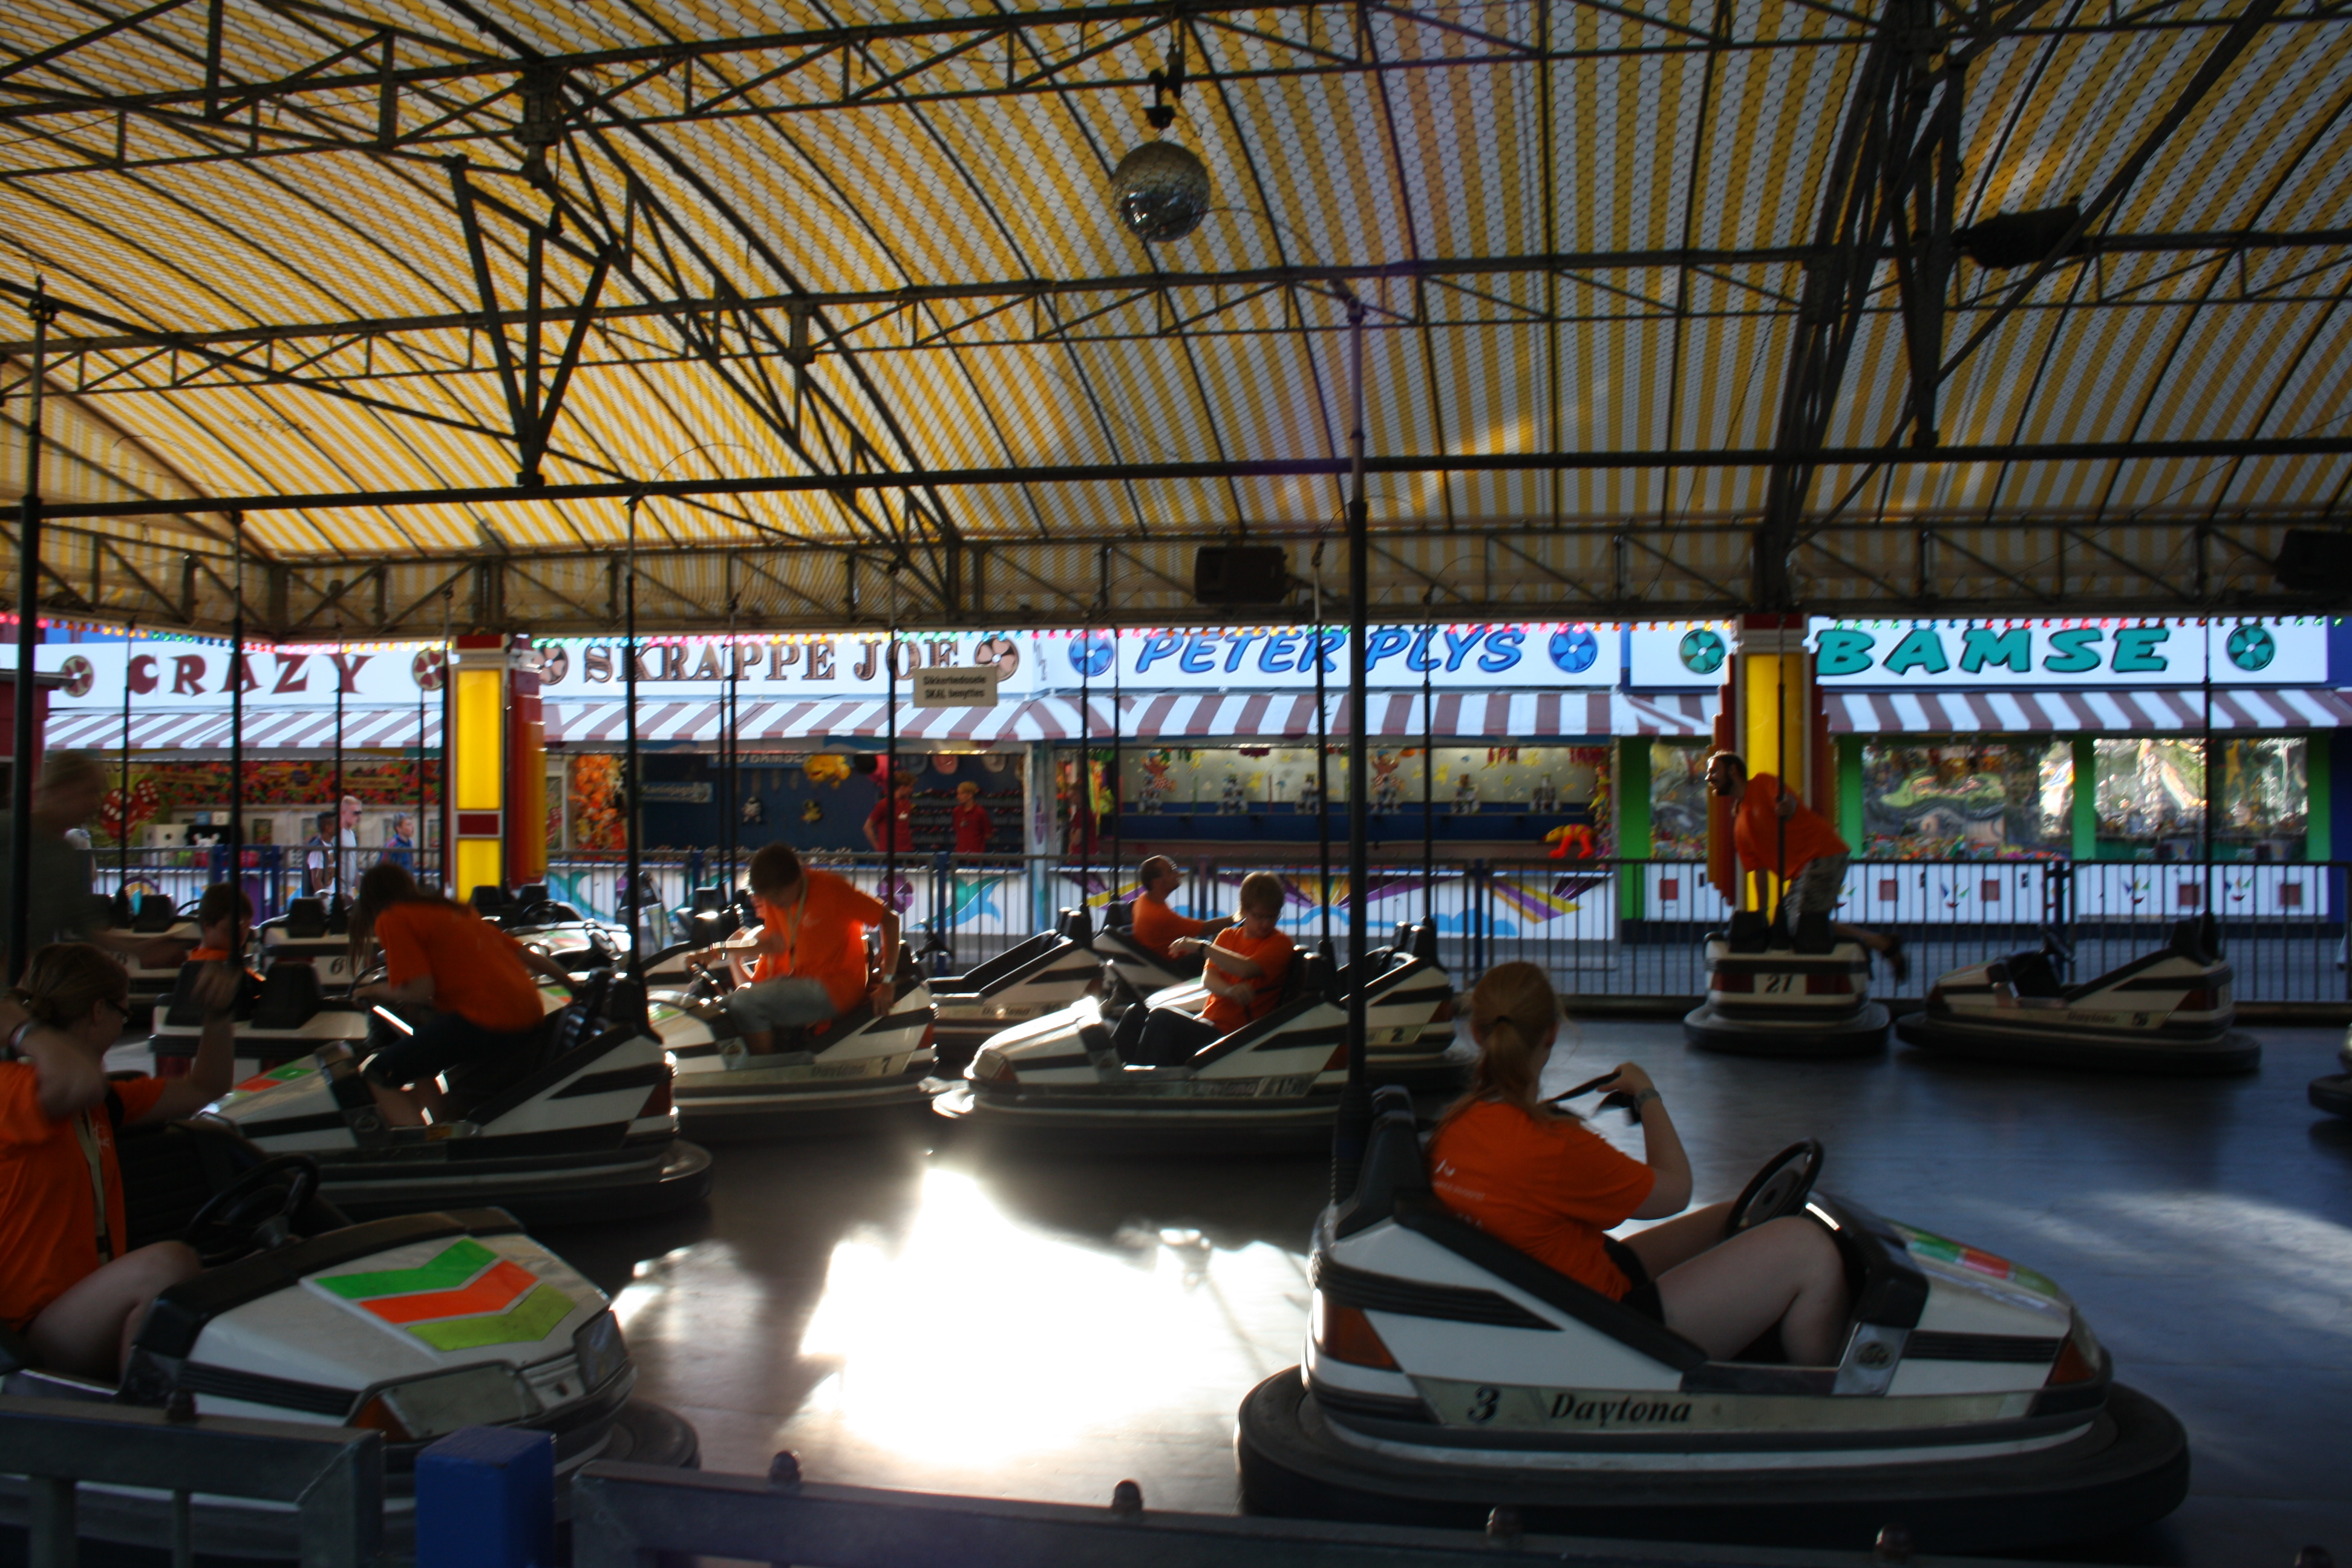
\includegraphics[width=\linewidth]{radiobil1.jpg}

\end{minipage}
